%% LyX 2.1.4 created this file.  For more info, see http://www.lyx.org/.
%% Do not edit unless you really know what you are doing.
\documentclass[12pt,a4paper]{article}
\usepackage{verbatim}
\usepackage{amsmath}
\usepackage{amsthm}
\usepackage{amssymb}
\usepackage{graphicx}
\usepackage{setspace}
\usepackage[numbers]{natbib}
\onehalfspacing

\makeatletter

%%%%%%%%%%%%%%%%%%%%%%%%%%%%%% LyX specific LaTeX commands.
\pdfpageheight\paperheight
\pdfpagewidth\paperwidth


%%%%%%%%%%%%%%%%%%%%%%%%%%%%%% Textclass specific LaTeX commands.
\numberwithin{equation}{section}
\numberwithin{figure}{section}

%%%%%%%%%%%%%%%%%%%%%%%%%%%%%% User specified LaTeX commands.
\usepackage{booktabs,multirow,array}
\newcolumntype{x}[1]{>{\centering\arraybackslash}m{#1}}

\@ifundefined{showcaptionsetup}{}{%
 \PassOptionsToPackage{caption=false}{subfig}}
\usepackage{subfig}
\makeatother

\begin{document}

\title{\textsf{Humans reciprocate intentional acts by discriminating against
group peers}}


\author{David Hugh-Jones, Itay Ron and Ro'i Zultan}
\maketitle
\begin{abstract}
Cycles of intergroup revenge appear in large scale conflicts. We experimentally
test the hypothesis that humans practice group-based reciprocity:
if someone harms or helps them, they harm or help other members of
that person's group. Subjects played a trust game, then allocated
money between other people. Senders whose partners returned more in
the trust game gave more to that partner's group members. The effect
was about 60 per cent of the size of the direct reciprocity effect.
Receivers' allocations to group members did not depend on their partner's
play, suggesting that group reciprocity was only triggered when the
partner's intentions were unequivocal.

\section{Introduction}

The evolution of cooperation poses a puzzle to evolutionary and social
scientists. Cooperation---by which individuals forgo personal benefits
to aid others---is a hallmark of human uniqueness. However, there
is a direct evolutionary pressure selecting against cooperators in
favour of free riders, who can reap the societal benefits of cooperation
without paying the costs. One mechanism that may underlie the evolution
of cooperation is reciprocity \citep{nowak2006five,nowak2012evolving}.
Direct reciprocity increases the fitness of cooperators, as helping
another individual leads to that individual reciprocating the help.
In indirect reciprocity, individuals help or harm other people than
those who have helped them.

Indirect reciprocity comes in two flavours: \emph{downstream} reciprocity
follows the maxim `do unto thy neighbour as they have done to others',
whereas \emph{upstream} reciprocity follows the maxim `do unto thy
neighbour as others have done unto you'. In this paper we study upstream
indirect reciprocity \citep{boyd1989evolution,nowak2005evolution,nowak2007upstream}.
Compared to downstream reciprocity, upstream reciprocity is simpler
to implement, as it does not require tracking individual reputations,
but is more difficult to understand from an evolutionary point of
view \citep{boyd1989evolution,nowak2005evolution}. Nonetheless, upstream
reciprocity can co-evolve with direct or spatial reciprocity \citep{nowak2007upstream}.
Furthermore, laboratory experiments provide positive evidence for
upstream reciprocity, as individuals are more generous to others if
a third party was generous to them \citep{dufwenberg2001direct,guth2001trust,greiner2005indirect},
and the mere possibility of being harmed by a third party reduces
cooperation in a social dilemma \citep{weisel2016social}. 

Direct and indirect reciprocity are embedded in a socially structured
world. Evidence suggests that human social behaviour---including cooperation
and reciprocity---is bounded by social groups \citep{tajfel1979integrative,yamagishi2000thegroup,balliet2014ingroup,DeDreu2014}.
Humans cooperate more with, and reciprocate more towards members of
their group \citep{chen2009group,chen2011potential}; and they punish
norm violators more if these harm a member of their own group \citep{bernhard2006group,bernhard2006parochial}.

Here we examine group-based upstream reciprocity, or \emph{group reciprocity}.
That is, an individual who is harmed (helped) by a member of an outgroup
becomes more likely to harm (help) others from that group. Whereas
group-based downstream reciprocity \citep{bernhard2006group,bernhard2006parochial}
follows the maxim `do unto others as they have done to members of
\emph{my} tribe', group-based upstream reciprocity follows the maxim
`do unto others as members of \emph{their} tribe have done to me'
(Figure~\ref{fig:illustration}). Both kinds of motive can expand
the scope of an individual-level conflict into an inter-group conflict.
While (group-based) downstream reciprocity can bring a victim's groupmates
in as retaliators, upstream reciprocity makes members of the aggressor's
group into potential targets. Ethnic conflicts provide ample evidence
that group identities play an important role in generalized reciprocity.
Humans take revenge on outgroups as well as on individuals, as evidenced
by the cycles of intergroup revenge that appear widespread in human
conflict \citep{horowitz2001thedeadly,horowitz1985ethnicgroups,chagnon1988lifehistories,shayo2010judicial}.
 

Upstream group reciprocity also has different cognitive requirements
from related phenomena. While in-group altruism and group-based downstream
reciprocity require people to differentiate their own group from outsiders---``us''
from ``them''---upstream group reciprocity requires them to differentiate
between different outgroups---between ``them and them''---and to
keep a mental account of outgroups' reputation. Upstream group reciprocity
could thus provide an evolutionary basis for the phenomenon of outgroup
stereotyping .
\end{abstract}
\begin{figure}
\subfloat[Someone who was helped or harmed becomes more likely to help or harm
new partners.]{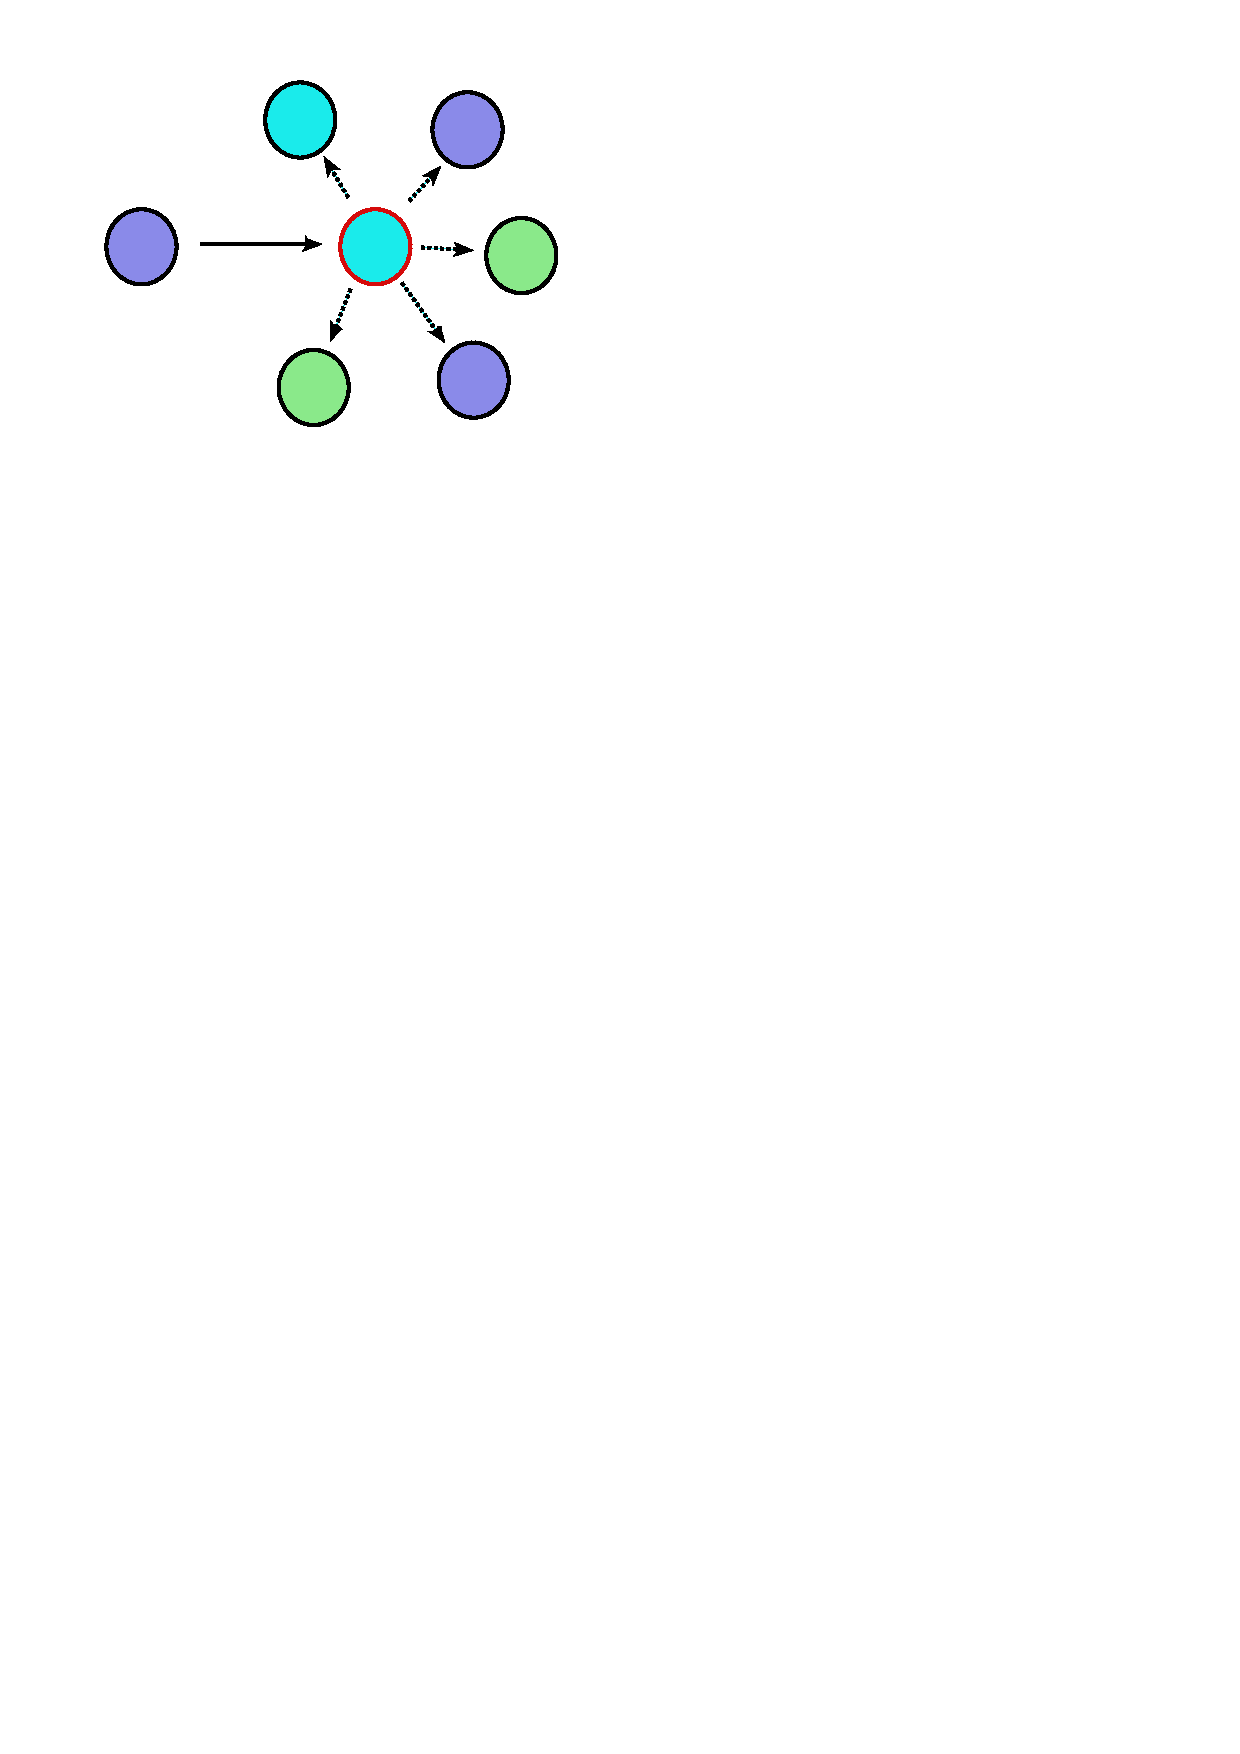
\includegraphics{upstream}

}

\subfloat[Group reciprocity: upstream reciprocity is particularly directed at
new partners that belong to the same group as the initial partner.]{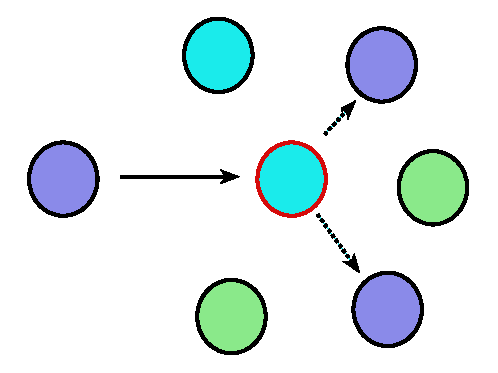
\includegraphics{group}

}

\caption{Indirect reciprocity}
\end{figure}

\begin{abstract}
We ran a laboratory experiment to test the hypothesis that people
reciprocate towards groups. After an initial group-formation stage,
participants interacted in two strategic stages. The first stage represented
the upstream interaction, in which the individual could be helped
by another person. We implemented this as a Trust Game (TG) \citep{berg1995trust},
in which the Sender~(S) receives~150 money-equivalent tokens, and
chooses how many of them to send to the Responder~(R). The amount
sent is multiplied by a factor of~3, so that R receives between 0~and~450
tokens, of which he can send any number back to S. The TG enables
us to model two types of interactions. Whereas R is clearly kind when
returning money (and nasty when exploiting a generous proposer by
keeping the received amount), S's intentions are equivocal. Sending
money can be driven by selfish expectations of reciprocity, while
not sending can be driven by caution. Thus,~R experiences kind or
nasty \emph{actions}, while~S experiences kind or nasty actions and
\emph{intentions}.

The second stage represented the reciprocal action, in which the individual
could help others. We implemented this interaction as an allocation
game, in which an allocator allocates a fixed amount between two recipients.
In Direct Reciprocity rounds, the recipients included the TG partner;
in Group Reciprocity rounds, a member of the TG partner's group; and
in In-Group Favouritism rounds, a member of the allocator's group.
The other recipient was always a member of a third, neutral, group.
Baseline rounds included two neutral recipients, to test whether the
TG experience lead allocators to discriminate in absence of any reciprocal
or group motivations. This design is an advance on previous work
\citep{gaertner2008whenrejection,stenstrom2008theroles,hugh-jones2013intergroup},
because it tests for group reciprocity using material incentives,
clearly differentiates the individual partner from his or her group
members, and rules out strategic motives.



\section{Method}

\label{sec:design}

Each session consisted of~24 participants, who were randomly allocated
into six groups of four. To distinguish from the groups in which participants
interacted throughout the different stages of the experiment, we refer
to the identity-relevant initial group as a \emph{Team}. Each participant
was identified throughout the experiment by team colour and individual
number (1--4) within the team. At the beginning of the experiment,
we informed participants that the experiment has five distinct stages.
In each stage, new groups are formed, and it is possible (though not
necessary) that two participants will be in the same group in two
different stages. The specific instructions for each stage were distributed
and read aloud at the beginning of the stage. The five stage were
a group formation stage, the TG stage, the AG stage, a social value
orientation elicitation \citep*{murphy2011measuring} stage and a
collectivism scale measurement \citep*[adapted from the horizontal collectivism scale in]{Singelis1995horizontal}.

Following \citet*{chen2009group}, we created group identity in the
first stage by allowing participants to consult each other using anonymous
chat while solving a simple task. Participants solved five Raven matrices
(see supplementary material). Each matrix was presented on screen
for 120~seconds, during which each participant could both send written
messages to the team and update her own answer. The final answer submitted
at the end of the 120~seconds determined payoffs, with 10~tokens
paid for each correct answer. To further boost group identity through
a common goal, team members each earned an additional bonus of 5~tokens
if all four team members answered correctly.

Next, participants were rematched into pairs to play the one-shot
TG. To facilitate understanding, participants played five practice
rounds, in which they entered decisions both as~S and as~R. In the
actual interaction, participants could see their TG partner's team
colour and individual number. The kindness of the Sender was measured
as the share of the endowment sent, and of the Responder as the share
of the received amount sent back. Responder's kindness was not defined
for six (out of 96) responders whose partner did not send any money.

The third stage consisted of six rounds. In each round, participants
interacted in a group of three, identified by team colour and number.
The allocation game was implemented as a random dictator game as follows.
Each player in the group of three received 100~tokens to allocate
within the group. The allocator received 30~tokens, and could freely
allocate the remaining 70~tokens between the other two players. Previous
research found that people do not harm, but refrain from helping negatively
perceived out-groups\citep{weisel2015ingroup}. Accordingly, we set
the parameters of the game so that, compared to the reference point
of the allocator's own share, an equal division benefits both other
players. The matching scheme ensured that over the six rounds, each
participant was in the same group of three exactly once with a member
of her own team (treatment IG), once with her TG partner (Treatment
DR), and twice with other members of the TG partner's team (treatment
GR). The remaining two rounds served as the baseline (B) treatment.
Note that the matching is not independent. For example, if one player
is in treatment DR, than the other two are in treatments DR and either
B or GR. No feedback was provided between rounds. The payoffs for
this stage were determined by one randomly chosen round of the six
rounds, and the allocation decision of one randomly chosen player
in each group.

The fourth stage implemented the slider measure of social value orientation
\citep*{murphy2011measuring,crosetto2012flexible}, in which participants
choose nine allocations between themselves and another person. For
consistency with the previous stages, the team identity of the partner
was known. To keep the decision independent of previous experience
with the different teams, we matched participants within teams. Consistently
with the notion of humans as parochial altruists, we believe that
such in-group allocations best reflect social preferences. Payoffs
were determined by one randomly chosen decision of the nine decisions
made by one randomly chosen player in each dyad. The decisions yielded
a social orientation angle for each participant, with~$0^{\circ}$
corresponding to selfishness, $45^{\circ}$ to pure altruism, and
negative angles to spitefulness.

After the fifth and final stage(a non-strategic and non-incentivised
collectivism measurement), participants learned their cumulative payoff
in tokens, and final payment in New Israeli Shekels. One hundred
and ninety two participants, recruited using ORSEE \citep*{greiner2015subject}
participated in eight sessions conducted between June 2014 and January
2015. Due to software malfunction in one session, the data from the
AG sixth round were not saved. The experiment was programmed in z-Tree
\citep*{Fischbacher2007}. The average payment was 72~NIS (approximately
\$18) for a duration of 70~minutes.

\section{Results}

\label{sec:results}

We report results on allocations, discrimination between recipients,
and direct and group reciprocity. All reported statistical tests are
based on mixed-effects regressions with robust standard errors clustered
on subjects. See the supplementary material for the full specification
and results.

\begin{table}[tbp] 
\begin{center} 
\def\sym#1{\ifmmode^{#1}\else\(^{#1}\)\fi} 
\caption{Allocations and discrimination \label{tab:results}} 
\begin{tabular}{p{4cm}*{3}{x{2.5cm}}} 
\toprule     
\multicolumn{4}{c}{Senders} \\     
\midrule     
                    &Discrimination         &Mean allocation         & Reciprocity         \\
\midrule
Baseline            &        4.06&       35.00&       0.00         \\
                    &      (0.99)         &      ---         &      ---         \\
Group               &        8.10\sym{***}&       34.58\sym{*}&        8.76\sym{**} \\
                    &      (1.73)         &      (0.78)         &      (4.34)         \\
Direct              &       22.13\sym{***}&       33.59\sym{*}&       13.89\sym{*}  \\
                    &      (2.84)         &      (1.82)         &      (7.95)         \\
In-Group            &       15.72\sym{***}&       39.25\sym{**}&        0.71         \\
                    &      (2.42)         &      (1.34)         &      (5.63)         \\
\midrule
Observations        &         564         &         728         &         728         \\
     
\midrule     
\multicolumn{4}{c}{Responders} \\     
\midrule     
                    &Discrimination         &Mean allocation         & Reciprocity         \\
\midrule
Baseline            &        2.14&       35.00&       0.00         \\
                    &      (0.64)         &      ---         &      ---         \\
Group               &        6.18\sym{***}&       34.59&        1.56         \\
                    &      (1.32)         &      (0.68)         &      (1.82)         \\
Direct              &       22.43\sym{***}&       35.47&       22.76\sym{***}\\
                    &      (2.83)         &      (1.63)         &      (4.59)         \\
In-Group            &       17.31\sym{***}&       41.76\sym{***}&        1.43         \\
                    &      (2.46)         &      (1.41)         &      (3.66)         \\
\midrule
Observations        &         564         &         752         &         752         \\
 
\bottomrule 
\multicolumn{4}{p{0.9\textwidth}}{
\footnotesize 
Notes: Mean discrimination, mean allocation, and reciprocity (marginal effect of TG partner's kindness on allocations) by recipient's identity. Estimates are based on mixed-effects regressions with robust standard errors clustered on subjects. Separate regressions for discrimination, Senders' allocations, and Responders' allocations.
Discrimination is higher than between two neutral players in all three experimental conditions. Allocations to in-group members are consistently higher than for a neutral player. Allocations to the TG partner strongly depend on his TG behavior. Allocations to the TG partner's team mates is dependent on his TG behavior only for Senders. Significance of comparison to Baseline is marked.
\sym{*}, \sym{**}, and \sym{***} indicate \(p<0.10\), \(p<0.05\), and \(p<0.01\), respectively.
}\\ 
\end{tabular} 
\end{center} 
\end{table} 

The second column in Table~\ref{tab:results} presents the mean allocations.
Participants gave significantly more to members of their own team
at the expense of the neutral recipient ($z=5.55,p<0.005$ for senders,
$z=4.79,p<0.001$ for responders), establishing that our group formation
manipulation was successful in inducing group identity and triggering
in-group favouritism. Allocations to the TG~partner and his team
mates were not significantly different to the baseline~35 ($p>0.440$
for all comparisons). Nonetheless, allocators discriminated significantly
more than in the baseline both when interacting with their TG partner
($z=9.36,p<0.001$) and with his team mates ($z=4.56,p<0.001),$as
reported in the first column of Table~\ref{tab:results}. The interaction
of the identity of the recipient and the allocator's TG role (sender
or receiver) was not significant ($\chi^{2}=1.42,p=0.700$).

\subsection*{Direct and group reciprocity}

\label{sec:reciprocity}

Figure~\ref{fig:reciprocity} presents the allocations made in the
DR and GR conditions separated by the whether the kindness of the
action of the TG partner was below the median or not. The median kindness
of the senders was~$\frac{1}{2}$ (median transfer of~75 out of~150
tokens). The median kindness of the responders was~$\frac{1}{3}$
(median share returned matches the amount sent). The figure reveals
strong direct reciprocity. Senders allocate less than the baseline~35
tokens to responders who failed to at least compensate the sender
for the amount sent. Responders both allocate more than~35 tokens
to senders who sent at least half their endowment, and less to those
who sent less. These observations are confirmed by the regression
analysis (see third column in Table~\ref{tab:results}). Allocations
to the TG partners increase with that partner's kindness both for
senders ($z=1.75,p=0.080$ and for responders ($z=4.96,p<0.001$).

Group reciprocity, however, is only observed for senders, who allocate
less to team mates of a responder who failed to at least compensate
the sender for the amount sent---a clear signal of bad intentions.
Responders, on the other hand, although directly reciprocating the
TG partner, do not systematically discriminate against team mates
of a sender who sent little---an unkind action that does not unequivocally
signals a bad intention. The regression analysis shows no significant
effect of sender kindness on responder's allocation to the sender's
team mates ($z=0.86,p=0.391$). The responder's kindness, on the other
hand, significantly increases allocations made to his team mates ($z=2.02,p<0.05$).
The estimated ratio of the group and direct reciprocity coefficients
is 0.63, implying that for every allocation dollar that the responder
loses due to an unkind action in the TG, his team mates lose~63 cents.

\begin{figure}
\caption{ Allocations made by to the TG partner (Direct Reciprocity) and his
team mates (Group Reciprocity) by TG partner's kindness with~95\%
confidence intervals based on subject-level averages. Responders give
more (less) to senders who sent more (less) then the median (equal
to exactly half the endowment)---but do not generalize to the sender's
team mates. Senders give less to responders who returned less than
the median (equal to exactly $\frac{1}{3}$, i.e., the amount sent)
and their team mates. }
\label{fig:reciprocity} 

\centering{}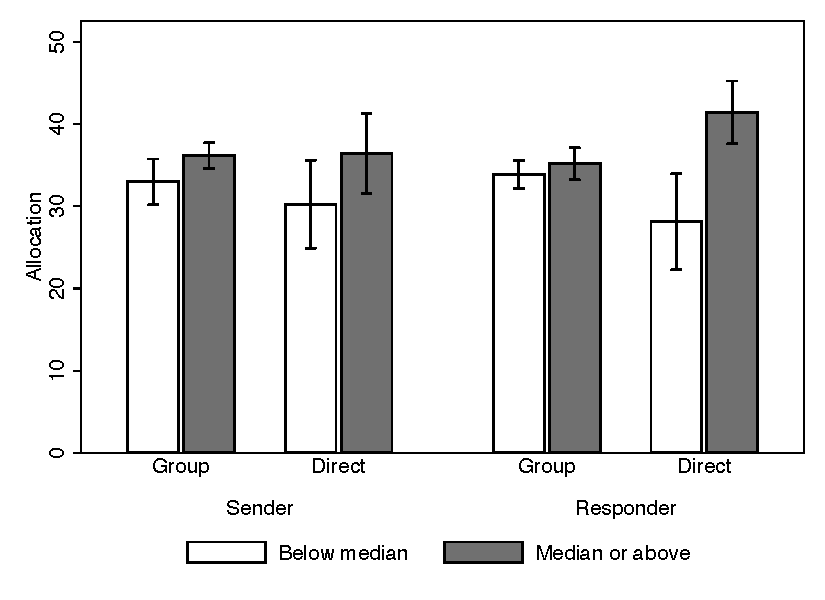
\includegraphics{Reciprocity} 
\end{figure}


\section{Discussion}

\label{sec:conclusion}

Our results show that upstream reciprocity is moderated by social
boundaries. We distinguish between two types of reciprocity: reciprocated
actions and reciprocated intentions \citep{stanca2009testing}. People
discriminate against others who harm them even if the harmful action
does not necessarily indicate bad intentions. However, they only generalize
to the perpetrator's  group members if the intentions behind the harmful
actions are unequivocally bad. 

This observation raises new questions regarding the nature of reciprocity
and the role of intentions (or perceptions thereof). One possible
interpretation stems from the distinction between intention-based
and outcome-based motives in reciprocal behaviour \citep{falk2006theory}.
Whereas intention-based reciprocity is plausibly generalisable, i.e.
subjects may wish to punish there is no reason to generalize outcome-based
reciprocity to group members who don't share the outcome. The notion
of outcome-based reciprocity is also related to that of restorative
justice. A desire to equalize earnings given the TG behaviour in the
experiment can motivate discrimination against a misbehaving TG partner,
but not his fellow group members.

A related distinction is between actions and types. Stereotypical
thinking can easily lead people to generalise types, whereas generalisation
of actions is nonsensical. The conjecture `One member of the Blue
group is a bad person, therefore all Blue members are bad' is plausible.
The conjecture `One member of the Blue group did not send any money,
therefore other Blue members did not send money' is not---as the other
Blue members did not even necessarily face the choice of how much
to send as a sender. 



Upstream reciprocity is notoriously difficult to understand in evolutionary
terms \citep{boyd1989evolution,nowak2007upstream} Group reciprocity
may provide another piece of the puzzle, as it provides two new channels
by which upstream reciprocity may evolve. First, group members are
interdependent, especially in the small groups that were the norm
during most of human evolutionary history. Punishing a perpetrator's
group member therefore indirectly harms the perpetrator, who is dependent
on his peers for, e.g., public goods provision. Thus, group reciprocity
may bridge upstream indirect reciprocity and direct reciprocity.

Second, the evolution of indirect reciprocity acts by way of chains
of reciprocal actions, which return with some probability to the original
instigator of the chain \citep{nowak2007upstream}. In a population
organised in groups, such that people interact more frequently with
their own group members, group reciprocity may increase the likelihood
of successful reciprocal chains, facilitating the evolution of upstream
reciprocity. We aim to explore these ideas in future work.

SUMMARY PARAGRAPH? WHAT DO WE WANT TO SAY ABOUT YAMAGISHI?

% Us and Them: we extend to Them and Them% Intentions generalize, actions don't% Possible evolutionary channels%
\begin{comment}
For example, we thought of it also as generalising types. It doesn't
make sense to punish Blue 2 for an action that he didn't do (Blue
1 did). The generalisation of if Blue 1 did something than all Blues
did it is clearly nonsensical. But if the motivation is to punish
bastards, it makes some sense to generalise that all blues are bastards
(well, 63\% percent they are :P), and therefore I should punish all
of them.
\end{comment}


\bibliographystyle{chicago}
\bibliography{grouprec}
\end{abstract}

\end{document}
